\documentclass[aspectratio=169,14pt]{beamer}
\usetheme{default}
\usepackage{fontspec}
\setmainfont{texgyrepagella-regular.otf}[BoldFont=texgyrepagella-bold.otf,ItalicFont=texgyrepagella-italic.otf,BoldItalicFont=texgyrepagella-bolditalic.otf]
\setsansfont{texgyreheros-regular.otf}[BoldFont=texgyreheros-bold.otf,ItalicFont=texgyreheros-italic.otf,BoldItalicFont=texgyreheros-bold.otf,BoldItalicFeatures={FakeSlant=0.2}]
\setmonofont{lmmono10-regular.otf}[Scale=0.85]
\setbeamertemplate{navigation symbols}{}
\usepackage{pgfpages}
\newif\ifpresenter
\ifdefined\PresenterVersion\presentertrue\else\presenterfalse\fi
\ifpresenter
  \setbeameroption{show notes on second screen=right}
  \setbeamertemplate{note page}[plain]
\fi
\usepackage{amsmath,amssymb,bm,booktabs,array,graphicx,xcolor}
\usepackage{tikz,pgfplots,adjustbox,listings,xurl}
\pgfplotsset{compat=1.18}
\usetikzlibrary{arrows.meta,positioning,calc,fit,shapes.geometric,decorations.pathreplacing,patterns}
% UIUC official brand colors, verified 2026-10-23.
% https://brand.illinois.edu/visual-identity/color
\definecolor{IlliniOrange}{HTML}{FF5F05}
\definecolor{IlliniBlue}{HTML}{13294B}
\definecolor{Storm}{HTML}{707372}
\definecolor{LightStorm}{HTML}{C6C7C6}
\definecolor{Industrial}{HTML}{1D58A7}
\definecolor{Patina}{HTML}{007E8E}
\tikzset{>=Stealth, every node/.style={font=\small,text=IlliniBlue}, box/.style={draw=IlliniBlue,rounded corners=2pt,align=center,inner sep=6pt,execute at begin node=\hyphenpenalty10000\relax}, orangebox/.style={box,draw=IlliniOrange,very thick}, edge/.style={->,thick,IlliniBlue}, accent/.style={->,very thick,IlliniOrange}}
\pgfplotsset{every axis/.append style={width=13.5cm,height=6.5cm,axis line style={IlliniBlue},tick label style={font=\small,text=IlliniBlue},label style={font=\small,text=IlliniBlue},legend style={font=\small,draw=none,fill=white},grid style={LightStorm},major grid style={LightStorm},axis lines=left,clip=false}, every axis plot/.append style={thick}}

\definecolor{slidepaper}{RGB}{234,220,201}
\setbeamercolor{background canvas}{bg=slidepaper}
\setbeamercolor{normal text}{fg=IlliniBlue}
\setbeamercolor{frametitle}{fg=IlliniBlue}
\setbeamercolor{title}{fg=IlliniBlue}
\setbeamercolor{item}{fg=IlliniOrange}
\setbeamerfont{frametitle}{size=\large,series=\bfseries}
\setbeamerfont{title}{size=\Large,series=\bfseries}
\setbeamertemplate{itemize item}{\color{IlliniOrange}$\bullet$}
\setbeamertemplate{itemize subitem}{\color{IlliniOrange}\footnotesize$\circ$}
\setbeamercolor{orangerule}{bg=IlliniOrange}
\setbeamertemplate{headline}{\begin{beamercolorbox}[wd=\paperwidth,ht=0.1cm,dp=0.1cm]{orangerule}\end{beamercolorbox}}
\setbeamertemplate{footline}{\begin{beamercolorbox}[wd=\paperwidth,ht=0.1cm,dp=0.1cm]{orangerule}\end{beamercolorbox}}
\setbeamersize{text margin left=0.65cm,text margin right=0.65cm}
\setlength{\leftmargini}{1.1em}
\newenvironment{slidebullets}{\begin{itemize}\setlength\itemsep{0.8em}}{\end{itemize}}
\pgfplotsset{every axis/.append style={legend style={fill=slidepaper}}}
\lstdefinelanguage{CoursePython}{keywords={from,import,for,in,if,else,def,return,assert,True,False,None},sensitive=true,morecomment=[l]{\#},morestring=[b]',morestring=[b]"}
\lstset{language=CoursePython,basicstyle=\ttfamily\small,keywordstyle=\color{IlliniBlue}\bfseries,commentstyle=\color{Storm},stringstyle=\color{IlliniBlue},showstringspaces=false,breaklines=true,columns=fullflexible,keepspaces=true,frame=none,aboveskip=0.7em,belowskip=0.7em}
\newcommand{\E}{\mathbb E}
\newcommand{\Var}{\operatorname{Var}}
\newcommand{\Cov}{\operatorname{Cov}}
\hypersetup{colorlinks=true,urlcolor=IlliniBlue,linkcolor=IlliniBlue}

\title{Marketing Analytics}
\subtitle{Prediction, Validation, and Marketing Actions}
\author{By Nathan Yang}
\date{Session 11}
\begin{document}
\begin{frame}
\titlepage
\end{frame}
\begin{frame}{A Service-Capacity Decision}
\usebeamercolor[fg]{normal text}
\vfill
\begin{slidebullets}
\item A team can review 100 customers each week.
\item Predictions use information available before that week.
\item The outcome and review benefit determine the useful metric.
\end{slidebullets}
\vfill
\note{A model selected on overall accuracy can fail to identify the cases that the team can help. The intervention value and the forecast are separate quantities.

M7, Section 7.1, Marketing Analytics Lecture Notes. \url{../06_Lecture_Notes/modules/M07_Prediction_and_Machine_Learning.md}}
\end{frame}
\begin{frame}{Validation Reproduces Deployment}
\usebeamercolor[fg]{normal text}
\centering
\begingroup
\fontsize{11}{13.2}\selectfont
\def\small{\fontsize{10}{12}\selectfont}
\def\footnotesize{\fontsize{9}{11}\selectfont}
\def\scriptsize{\fontsize{8}{9.5}\selectfont}
\hyphenpenalty=10000
\begin{adjustbox}{max width=0.98\textwidth,max totalheight=0.65\textheight}
% Original synthetic teaching figure; see corresponding module.
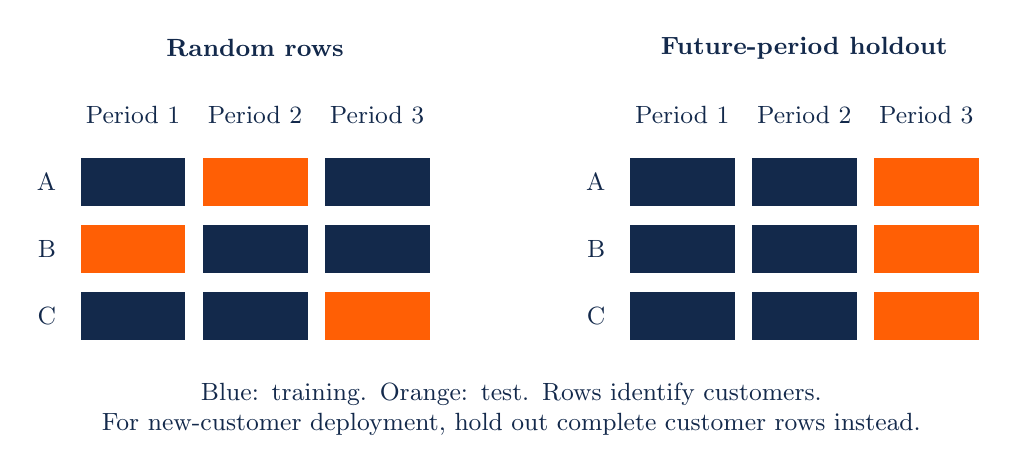
\begin{tikzpicture}[x=1.55cm,y=.85cm]
\foreach \x/\lab in {0/Period 1,1/Period 2,2/Period 3} {\node at (\x,1) {\lab};\node at (\x+4.5,1) {\lab};}
\node[font=\small\bfseries] at (1,2) {Random rows};\node[font=\small\bfseries] at (5.5,2) {Future-period holdout};
\foreach \y/\lab in {0/A,-1/B,-2/C} {\node[anchor=east] at (-.55,\y) {\lab};\node[anchor=east] at (3.95,\y) {\lab};}
\foreach \x/\y in {0/0,2/0,1/-1,2/-1,0/-2,1/-2} {\fill[IlliniBlue] (\x-.43,\y-.36) rectangle (\x+.43,\y+.36);}
\foreach \x/\y in {1/0,0/-1,2/-2} {\fill[IlliniOrange] (\x-.43,\y-.36) rectangle (\x+.43,\y+.36);}
\foreach \x in {4.5,5.5} {\foreach \y in {0,-1,-2} {\fill[IlliniBlue] (\x-.43,\y-.36) rectangle (\x+.43,\y+.36);}}
\foreach \y in {0,-1,-2} {\fill[IlliniOrange] (6.07,\y-.36) rectangle (6.93,\y+.36);}
\node[align=center,text width=12cm] at (3.1,-3.4) {Blue: training. Orange: test. Rows identify customers.\\For new-customer deployment, hold out complete customer rows instead.};
\end{tikzpicture}

\end{adjustbox}
\endgroup
\par\medskip
{\small The deployment population determines the appropriate holdout.\par}
\note{New-customer prediction requires separation by customer. Future prediction for returning customers requires separation in time. Some deployments require both.

M7, Section 7.4, Marketing Analytics Lecture Notes. \url{../06_Lecture_Notes/modules/M07_Prediction_and_Machine_Learning.md}}
\end{frame}
\begin{frame}{Selection on Development Accuracy}
\usebeamercolor[fg]{normal text}
\centering
\begingroup
\begin{adjustbox}{max width=0.98\textwidth,max totalheight=0.65\textheight}
\begin{tikzpicture}
\begin{axis}[width=12cm,height=6.4cm,xmode=log,log basis x=10,xmin=.8,xmax=125,
ymin=45,ymax=70,xtick={1,5,20,100},xticklabels={1,5,20,100},
ytick={45,50,55,60,65,70},xlabel={Candidates Compared},ylabel={Expected Accuracy (\%)},
ymajorgrids=true,legend style={at={(.5,1.03)},anchor=south,legend columns=2,fill=none}]
\addplot[IlliniOrange,mark=square*,mark size=3pt] table[col sep=comma,x=candidates,
y expr=100*\thisrow{expected_development_accuracy}]
{../03_Data_and_Code/AI_Workflows/results/selection_results.csv};
\addlegendentry{Selected Development}
\addplot[IlliniBlue,dashed,mark=*,mark size=3pt] table[col sep=comma,x=candidates,
y expr=100*\thisrow{expected_test_accuracy}]
{../03_Data_and_Code/AI_Workflows/results/selection_results.csv};
\addlegendentry{Fresh Test}
\end{axis}
\end{tikzpicture}

\end{adjustbox}
\endgroup
\par\medskip
{\small Synthetic independent chance predictions: 80 development cases per candidate.\par}
\note{Each candidate has true accuracy one-half under the imposed independent Bernoulli model. The maximum development score increases with the number compared. Fresh test correctness is independent of selection. The program verifies the analytic expectation and simulates 2,000 repetitions with 200 test cases. Real prompt candidates can be correlated, so the magnitude is illustrative.

Marketing Analytics Lecture Notes, M7 §7.20.}
\end{frame}
\begin{frame}{The Forecast Origin}
\usebeamercolor[fg]{normal text}
\vfill
\begin{slidebullets}
\item Features end before the decision time.
\item The outcome window begins after the decision.
\item Training labels must already be observable at fitting time.
\end{slidebullets}
\vfill
\note{A database extract can contain information that did not exist at the historical prediction origin. Store measurement windows or feature timestamps to make the information constraint verifiable.

M7, Section 7.1, Marketing Analytics Lecture Notes. \url{../06_Lecture_Notes/modules/M07_Prediction_and_Machine_Learning.md}}
\end{frame}
\begin{frame}{Baselines and Model Families}
\usebeamercolor[fg]{normal text}
\vfill
\begin{slidebullets}
\item Compare with a constant probability or recent-history forecast.
\item Logistic regression supplies a probability baseline.
\item Trees represent conditional splits. Ensembles combine trees.
\end{slidebullets}
\vfill
\note{A complex model earns its place through performance on the intended held-out observations and decision costs. Training fit alone rewards flexibility.

M7, Section 7.2, Marketing Analytics Lecture Notes. \url{../06_Lecture_Notes/modules/M07_Prediction_and_Machine_Learning.md}}
\end{frame}
\begin{frame}{Logistic Prediction}
\usebeamercolor[fg]{normal text}
\noindent Transform a linear index into a binary-outcome probability.
\medskip
\[
\widehat p_i=\frac{1}{1+\exp[-(\beta_0+x_i^\top\beta)]}
\]
\medskip
\noindent A coefficient changes log odds. Its probability effect depends on the starting point.
\note{The same index change has a larger probability effect near the middle than near zero or one. Calibration should be evaluated on the deployment population.

M7, Section 7.3, Marketing Analytics Lecture Notes. \url{../06_Lecture_Notes/modules/M07_Prediction_and_Machine_Learning.md}}
\end{frame}
\begin{frame}{Preprocessing Belongs in Training}
\usebeamercolor[fg]{normal text}
\vfill
\begin{slidebullets}
\item Fit imputation, scaling, and vocabulary on training records.
\item Choose model settings using validation data.
\item Keep the final test sample separate from model selection.
\end{slidebullets}
\vfill
\note{Repeatedly choosing features from test performance turns that sample into validation data. A pipeline helps preserve the training-only boundary within cross-validation.

M7, Section 7.4, Marketing Analytics Lecture Notes. \url{../06_Lecture_Notes/modules/M07_Prediction_and_Machine_Learning.md}}
\end{frame}
\begin{frame}{Rare Purchases and Accuracy}
\usebeamercolor[fg]{normal text}
\vfill
\centering
{\small\begin{tabular}{lrr}
\toprule
Quantity & Flagged & Not Flagged \\
\midrule
Purchases & 30 & 20 \\
No Purchase & 70 & 880 \\
\bottomrule
\end{tabular}}
\par\medskip
Synthetic population: 1,000 customers and 50 purchases.
\vfill
\note{Flagging 100 customers gives precision 30\%, recall 60\%, and accuracy 91\%. Predicting no purchase for everybody gives 95\% accuracy and finds no purchasers.

M7, Section 7.5, Marketing Analytics Lecture Notes. \url{../06_Lecture_Notes/modules/M07_Prediction_and_Machine_Learning.md}}
\end{frame}
\begin{frame}{Metrics and the Review Queue}
\usebeamercolor[fg]{normal text}
\vfill
\begin{slidebullets}
\item Precision: what fraction of reviewed cases are positive?
\item Recall: what fraction of positives enter the queue?
\item Calibration: do predicted probabilities match observed frequencies?
\end{slidebullets}
\vfill
\note{The appropriate contact fraction should match staff capacity. A ranking measure and a probability measure answer different questions. Neither by itself measures the causal effect of contacting a customer.

M7, Section 7.6, Marketing Analytics Lecture Notes. \url{../06_Lecture_Notes/modules/M07_Prediction_and_Machine_Learning.md}}
\end{frame}
\begin{frame}{Ranking Can Stay Fixed While Probabilities Change}
\usebeamercolor[fg]{normal text}
\centering
\begingroup
\begin{adjustbox}{max width=0.98\textwidth,max totalheight=0.65\textheight}
% Original synthetic teaching figure; see corresponding module.
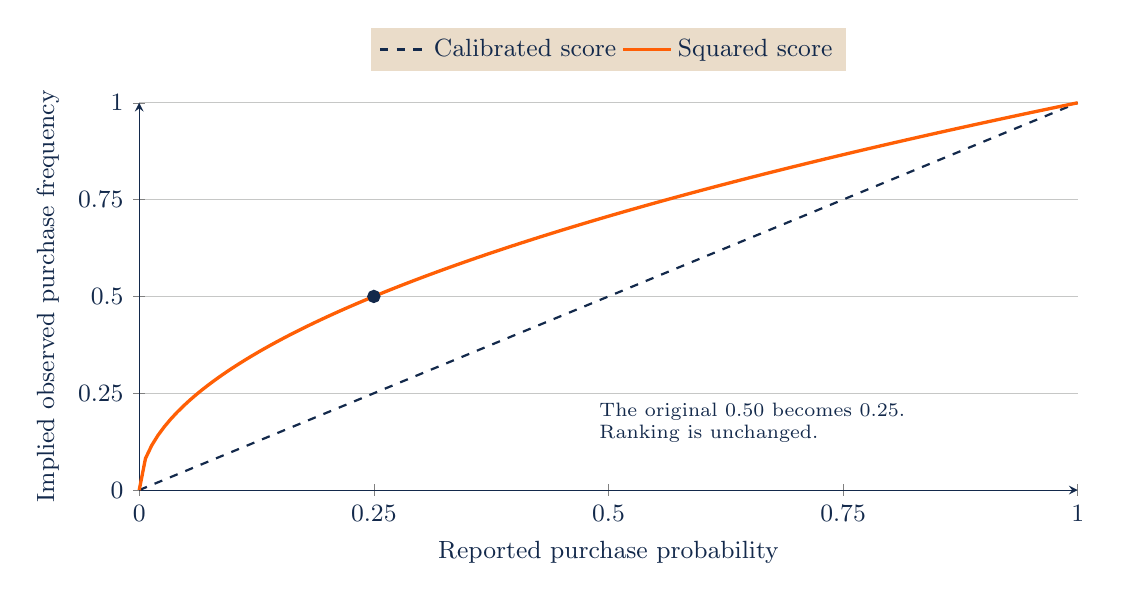
\begin{tikzpicture}
\begin{axis}[xmin=0,xmax=1,ymin=0,ymax=1,xlabel={Reported purchase probability},ylabel={Implied observed purchase frequency},xtick={0,.25,.5,.75,1},ytick={0,.25,.5,.75,1},legend style={at={(.5,1.08)},anchor=south,legend columns=2},ymajorgrids=true]
\addplot[IlliniBlue,dashed,domain=0:1] {x};
\addplot[IlliniOrange,very thick,domain=0:1,samples=151] {sqrt(x)};
\legend{Calibrated score,Squared score}
\addplot[IlliniBlue,only marks,mark=*] coordinates {(.25,.5)};
\node[align=left,anchor=north west,font=\scriptsize] at (axis cs:.48,.25) {The original 0.50 becomes 0.25.\\Ranking is unchanged.};
\end{axis}
\end{tikzpicture}

\end{adjustbox}
\endgroup
\par\medskip
{\small A synthetic transformation squares initially calibrated probabilities.\par}
\note{For q=p squared, the original outcome frequency p equals the square root of q. Expected contribution calculations need probabilities with the relevant interpretation.

M7, Section 7.6, Marketing Analytics Lecture Notes. \url{../06_Lecture_Notes/modules/M07_Prediction_and_Machine_Learning.md}}
\end{frame}
\begin{frame}{Identical Ranking, Different Probabilities}
\usebeamercolor[fg]{normal text}
\centering
\begingroup
\begin{adjustbox}{max width=0.98\textwidth,max totalheight=0.65\textheight}
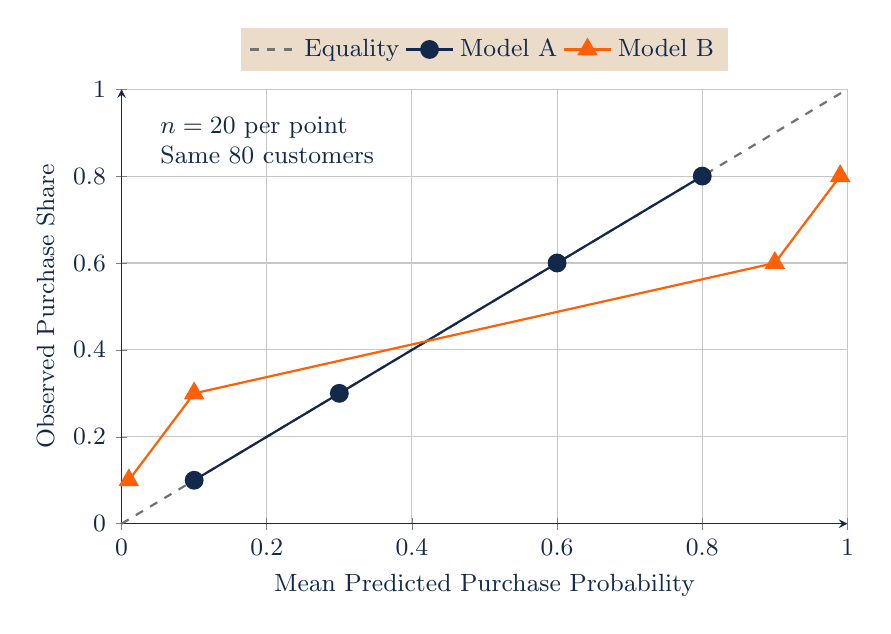
\begin{tikzpicture}
\begin{axis}[width=10.8cm,height=7.1cm,xmin=0,xmax=1,ymin=0,ymax=1,
xtick={0,.2,.4,.6,.8,1},ytick={0,.2,.4,.6,.8,1},
xlabel={Mean Predicted Purchase Probability},ylabel={Observed Purchase Share},
grid=major,legend style={at={(.5,1.04)},anchor=south,legend columns=3,
font=\small,cells={anchor=west}},
legend cell align=left]
\addplot[Storm,dashed,no marks] coordinates {(0,0) (1,1)};
\addlegendentry{Equality}
\addplot[IlliniBlue,mark=*,mark size=3pt] coordinates {(.1,.1) (.3,.3) (.6,.6) (.8,.8)};
\addlegendentry{Model A}
\addplot[IlliniOrange,mark=triangle*,mark size=3.5pt] coordinates {(.01,.1) (.1,.3) (.9,.6) (.99,.8)};
\addlegendentry{Model B}
\node[anchor=north west,align=left,font=\small] at (axis cs:.04,.96) {$n=20$ per point\\Same 80 customers};
\end{axis}
\end{tikzpicture}

\end{adjustbox}
\endgroup
\par\medskip
{\small Synthetic customers and imposed scores: both models have AUC 0.803. Each plotted group contains 20 customers.\par}
\note{The same 80 eligible customers have 36 purchases and 44 nonpurchases in one next-month window. Each can purchase at most once. Group calibration of Model A is imposed; no trained model or future performance claim is involved. No uncertainty interval is attached to this fixed constructed population.

M7 Section 7.23. \url{../06_Lecture_Notes/modules/M07_Prediction_and_Machine_Learning.md}}
\end{frame}
\begin{frame}{AUC Alone Does Not Set Inventory}
\usebeamercolor[fg]{normal text}
\vfill
\centering
{\small\begin{tabular}{lrr}
\toprule
Quantity & Model A & Model B \\
\midrule
AUC & 0.803 & 0.803 \\
Brier Score & 0.175 & 0.21855 \\
Predicted Purchases & 36 & 40 \\
Observed Purchases & 36 & 36 \\
\bottomrule
\end{tabular}}
\par\medskip
Same 80 synthetic customers. Smaller Brier scores indicate less squared probability error.
\vfill
\note{AUC gives half credit to tied positive-negative pairs: 1272/1584 = 53/66 for both models. A strictly increasing score transformation preserves ordering. The sum of probabilities changes, making probability accuracy relevant to inventory. The Brier score is an overall probability loss, not solely a calibration measure. Purchase propensity does not identify a coupon effect.

\url{../03_Data_and_Code/Statistical_Graphics/README.md} \url{https://warint.github.io/pystatlas/model-diagnostics/calibration-plot/}}
\end{frame}
\begin{frame}{A Cost-Based Threshold}
\usebeamercolor[fg]{normal text}
\noindent Suppose false positives cost $C_{FP}$ and false negatives cost $C_{FN}$.
\medskip
\[
p>\frac{C_{FP}}{C_{FP}+C_{FN}}
\]
\medskip
\noindent With costs 1 and 9, the threshold is 0.10 under this simplified classification loss.
\note{Correct classifications have zero cost in this example. Capacity constraints and different action effects require a richer decision model.

M7, Section 7.7, Marketing Analytics Lecture Notes. \url{../06_Lecture_Notes/modules/M07_Prediction_and_Machine_Learning.md}}
\end{frame}
\begin{frame}{Coupon Targeting Includes the Untreated Outcome}
\usebeamercolor[fg]{normal text}
\centering
\begingroup
\begin{adjustbox}{max width=0.98\textwidth,max totalheight=0.65\textheight}
% Original synthetic teaching figure; see corresponding module.
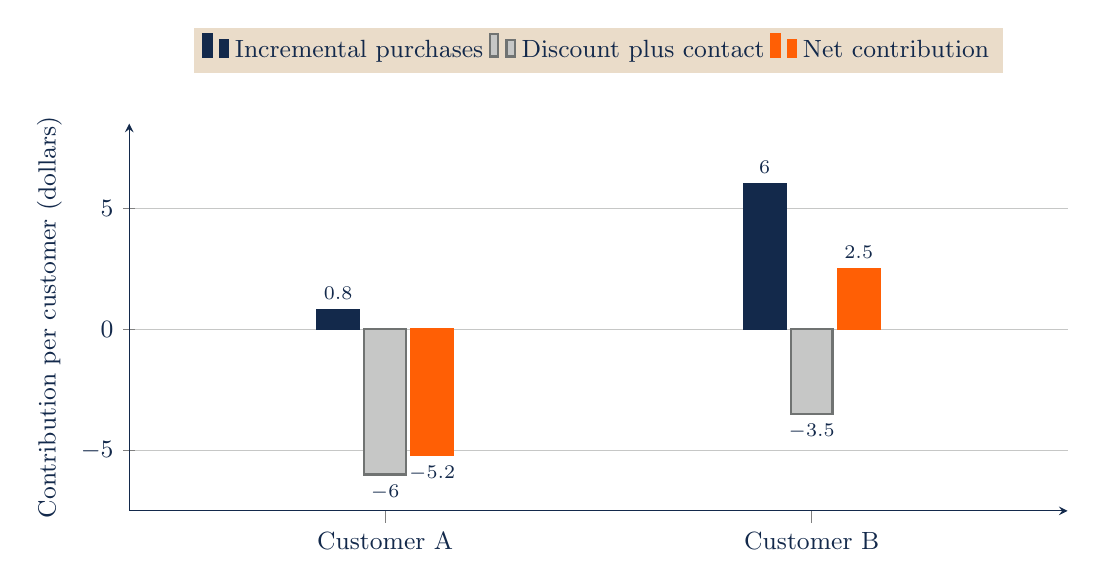
\begin{tikzpicture}
\begin{axis}[ybar,bar width=15pt,xmin=.4,xmax=2.6,ymin=-7.5,ymax=8.5,xtick={1,2},xticklabels={Customer A,Customer B},ylabel={Contribution per customer (dollars)},ymajorgrids=true,legend style={at={(.5,1.13)},anchor=south,legend columns=3},nodes near coords,nodes near coords style={font=\scriptsize}]
\addplot[fill=IlliniBlue,draw=IlliniBlue] coordinates {(1,.8)(2,6)};
\addplot[fill=LightStorm,draw=Storm] coordinates {(1,-6)(2,-3.5)};
\addplot[fill=IlliniOrange,draw=IlliniOrange] coordinates {(1,-5.2)(2,2.5)};
\legend{Incremental purchases,Discount plus contact,Net contribution}
\end{axis}
\end{tikzpicture}

\end{adjustbox}
\endgroup
\par\medskip
{\small Synthetic probabilities and costs. High treated response can have negative incremental value.\par}
\note{Contribution is 40 dollars, discount 5 dollars per treated purchase, and contact cost 2 dollars. Baseline probabilities are 0.78 and 0.15. Discount expense applies to purchases that would also have occurred without the coupon.

M7, Section 7.8, Marketing Analytics Lecture Notes. \url{../06_Lecture_Notes/modules/M07_Prediction_and_Machine_Learning.md}}
\end{frame}
\begin{frame}[fragile]{Queue Metrics}
\usebeamercolor[fg]{normal text}
\noindent Compute metrics from the synthetic confusion matrix.
\begin{lstlisting}
tp, fn, fp, tn = 30, 20, 70, 880
precision = tp / (tp + fp)
recall = tp / (tp + fn)
accuracy = (tp + tn) / (tp + fn + fp + tn)
assert (precision, recall, accuracy) == (0.3, 0.6, 0.91)
\end{lstlisting}
{\small The model finds 60\% of purchasers while 70\% of its queue contains nonpurchasers.\par}
\note{Whether that queue is profitable depends on the action and its incremental outcome. A prediction score alone cannot supply the causal response to a coupon.

M7, Section 7.5, Marketing Analytics Lecture Notes. \url{../06_Lecture_Notes/modules/M07_Prediction_and_Machine_Learning.md}}
\end{frame}
\begin{frame}{McBroken Forecasting}
\usebeamercolor[fg]{normal text}
\vfill
\begin{slidebullets}
\item Predict availability on a later date.
\item Retain a separate count of unknown future labels.
\item Compare baseline and fitted forecasts on the same observed outcomes.
\end{slidebullets}
\vfill
\note{An unknown future status is not an observed available restaurant. Dropping missing labels changes the evaluated population and can make an apparently strong forecast depend on observation coverage.

M7, Section 7.18, Marketing Analytics Lecture Notes. \url{../06_Lecture_Notes/modules/M07_Prediction_and_Machine_Learning.md}}
\end{frame}
\begin{frame}{Prediction and Outcome Coverage}
\usebeamercolor[fg]{normal text}
\centering
\begingroup
\begin{adjustbox}{max width=0.98\textwidth,max totalheight=0.65\textheight}
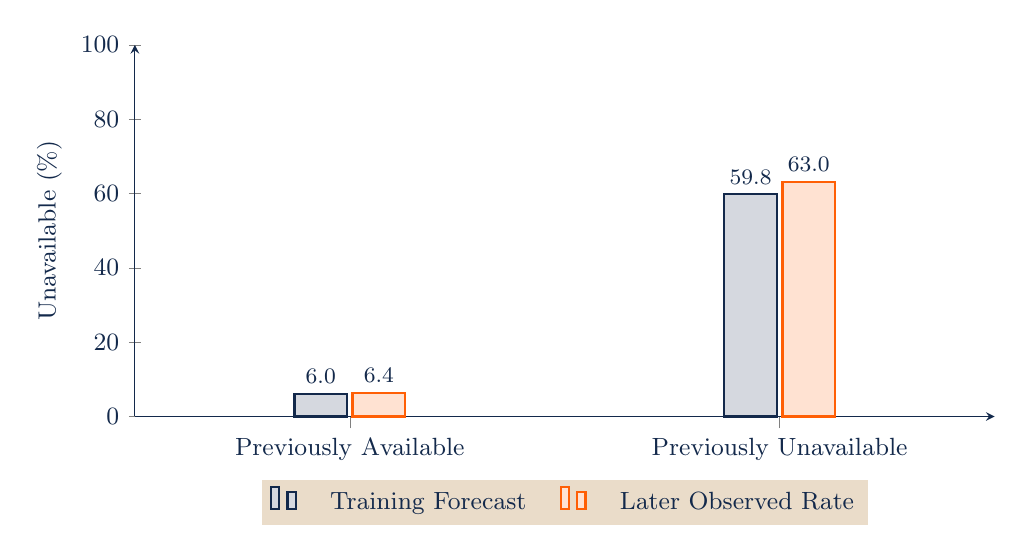
\begin{tikzpicture}
\begin{axis}[ybar,bar width=19pt,width=12.5cm,height=6.3cm,ymin=0,ymax=100,
 ylabel={Unavailable (\%)},xtick={0,1},xticklabels={Previously Available,Previously Unavailable},
 enlarge x limits=0.5,legend style={at={(0.5,-0.17)},anchor=north,legend columns=2,column sep=10pt},
 nodes near coords,every node near coord/.append style={font=\footnotesize,/pgf/number format/fixed,/pgf/number format/fixed zerofill,/pgf/number format/precision=1}]
\addplot[draw=IlliniBlue,fill=IlliniBlue!18] coordinates {(0,5.968281) (1,59.779013)};
\addplot[draw=IlliniOrange,fill=IlliniOrange!18] coordinates {(0,6.354498) (1,63.027663)};
\legend{Training Forecast,Later Observed Rate}
\end{axis}
\end{tikzpicture}

\end{adjustbox}
\endgroup
\par\medskip
{\small McBroken forecasts use later dates and observed-label denominators.\par}
\note{The course example checks information availability at the forecast origin and uses chronological evaluation. Missing outcome counts remain alongside accuracy measures.

M7, Section 7.18.2, Marketing Analytics Lecture Notes. \url{../06_Lecture_Notes/modules/M07_Prediction_and_Machine_Learning.md}}
\end{frame}
\begin{frame}{Accuracy and Failure Costs}
\usebeamercolor[fg]{normal text}
\centering
\begingroup
\begin{adjustbox}{max width=0.98\textwidth,max totalheight=0.65\textheight}
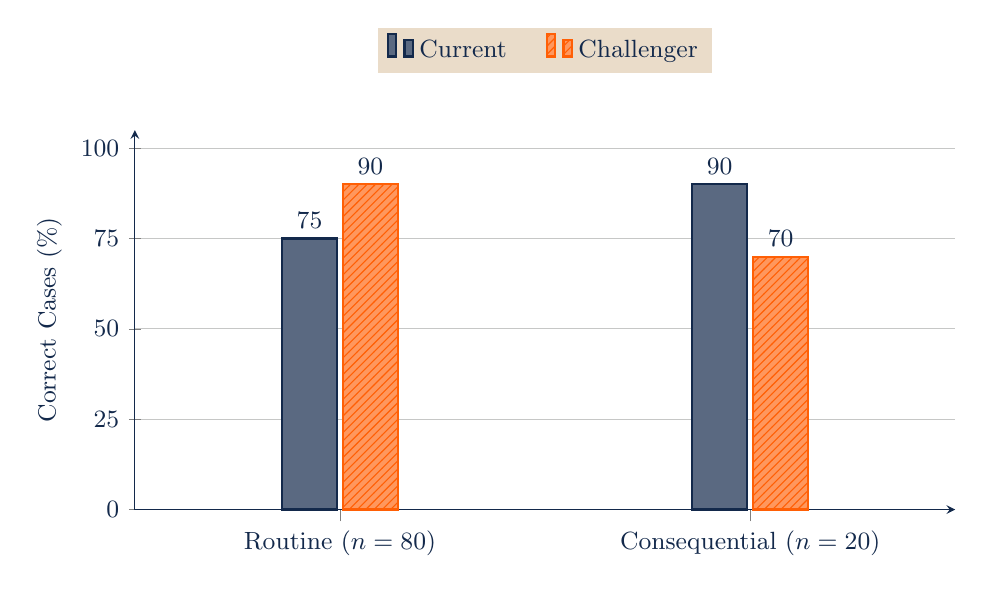
\begin{tikzpicture}
\begin{axis}[ybar,width=12cm,height=6.4cm,ymin=0,ymax=105,
ytick={0,25,50,75,100},ylabel={Correct Cases (\%)},
symbolic x coords={Routine,Consequential},xtick=data,
xticklabels={Routine ($n=80$),Consequential ($n=20$)},
bar width=20pt,enlarge x limits=.5,ymajorgrids=true,
nodes near coords,nodes near coords style={font=\small},
legend style={at={(.5,1.15)},anchor=south,legend columns=2,
cells={anchor=west},/tikz/every even column/.append style={column sep=12pt}}]
\addplot[fill=IlliniBlue!70,draw=IlliniBlue] coordinates {(Routine,75) (Consequential,90)};
\addplot[fill=IlliniOrange!65,draw=IlliniOrange,postaction={pattern=north east lines,pattern color=IlliniOrange}] coordinates {(Routine,90) (Consequential,70)};
\legend{Current,Challenger}
\end{axis}
\end{tikzpicture}

\end{adjustbox}
\endgroup
\par\medskip
{\small Constructed cases: pooled accuracy rises from 78\% to 86\%.\par}
\note{Fourteen paired cases improve and six regress. Stipulated failure costs of one dollar for routine tasks and twenty dollars for consequential tasks give losses of sixty and 128 dollars. The additional four consequential failures outweigh the twelve avoided routine failures. These are constructed values, not measured model performance.

M7 §7.22. \url{../03_Data_and_Code/LLM_Revalidation/README.md}}
\end{frame}
\begin{frame}[fragile]{Paired Regression Checks}
\usebeamercolor[fg]{normal text}
\noindent The same one hundred constructed cases are scored under both configurations.
\begin{lstlisting}
improved, regressed, cases = 14, 6, 100
gain_pp = 100 * (improved - regressed) / cases
old_loss = 20 * 1 + 2 * 20
new_loss = 8 * 1 + 6 * 20
print(gain_pp, old_loss, new_loss)
\end{lstlisting}
{\small Output: 8.0 percentage points; current loss 60 dollars; challenger loss 128 dollars.\par}
\note{The complete program preserves every paired case and each segment denominator. With a consequential-to-routine loss ratio q, the change in failure loss is -12 + 4q. The challenger improves this loss only below a ratio of three. Inference fees, setup costs, and other outcomes require additional terms.

M7 §7.22. \url{../03_Data_and_Code/LLM_Revalidation/evaluate_upgrade.py}}
\end{frame}
\begin{frame}{Coding Exercise: A Forecast Evaluation}
\usebeamercolor[fg]{normal text}
\vfill
\begin{slidebullets}
\item Compare development and fresh accuracy after candidate selection.
\item Check every feature against the forecast date.
\item Compare a simple baseline, ranking, and calibration.
\item Report missing outcomes beside the test metrics.
\end{slidebullets}
\vfill
\note{Run ../03\_Data\_and\_Code/Lecture\_Examples/session\_examples.py S11 for the metrics example. Use the McBroken forecasting scripts for the real-panel extension, following their README and saved outcome definitions. The AI\_Workflows folder supplies complete standard-library calculations with synthetic inputs.

M7, Section 7.14, Marketing Analytics Lecture Notes. \url{../06_Lecture_Notes/modules/M07_Prediction_and_Machine_Learning.md}}
\end{frame}
\begin{frame}{Targeting and Delivered Opportunities}
\usebeamercolor[fg]{normal text}
\vfill
\begin{slidebullets}
\item An apparently neutral target can produce unequal delivery.
\item Evaluate exposure and error costs across relevant groups.
\item Housing, credit, and employment applications require their specific legal context.
\end{slidebullets}
\vfill
\note{The DOJ's Meta housing-ad settlement addresses discriminatory delivery as well as targeting tools. That case is evidence about housing advertising and should not be generalized into a single rule for all products.

DOJ, United States v. Meta Platforms. \url{https://www.justice.gov/crt/case/united-states-v-meta-platforms-inc-fka-facebook-inc-sdny}}
\end{frame}
\begin{frame}{Prediction Discussion}
\usebeamercolor[fg]{normal text}
\vfill
\begin{slidebullets}
\item Which error uses scarce review capacity?
\item Which feature becomes available too late?
\item Does the score support a forecast, an intervention, or both?
\end{slidebullets}
\vfill
\note{A deployment decision needs an explicit chain from information to prediction to action. Each link has its own empirical requirements.

M7, Section 7.9, Marketing Analytics Lecture Notes. \url{../06_Lecture_Notes/modules/M07_Prediction_and_Machine_Learning.md}}
\end{frame}
\end{document}
